%%%%%%%%%%%%%%%%%%%%%%%%%%%%%%%%%%%%%%%%%%%%%%%%%%%%%%%%%%%%%%%%%%%%%%
% Lớp 12 | Ứng dụng đạo hàm để khảo sát hàm số | Cực trị của hàm số
% Dạng 2D1?2-7: Toán thực tế ứng dụng cực trị của hàm số
% Số câu: 19  (sinh tự động bởi tach_cau.py; từ nay thầy sửa trực tiếp file này)
%%%%%%%%%%%%%%%%%%%%%%%%%%%%%%%%%%%%%%%%%%%%%%%%%%%%%%%%%%%%%%%%%%%%%%

%%%%%%%%%%%%%%%% TRẮC NGHIỆM 4 PHƯƠNG ÁN %%%%%%%%%%%%%%%%

% nguồn: Phan1_Lop_12_Dai_so_Chuong_1
\begin{ex}%[2D1H2-7]%[ma:3b998964]
	Độ giảm huyết áp của một bệnh $G(x)=0{,}025x^2(30-x)$ trong đó $x$  là số miligam thuốc được tiêm cho bệnh nhân $(0<x<30)$. Để bệnh nhân đó có huyết áp giảm nhiều nhất thì liều lượng thuốc cần tiêm vào là
	 \choice
		 {$x=15$ (mg)}
		 {$x=10$ (mg)}
		{\True $x=20$ (mg)} 
		 {$x=25$ (mg)}
	\loigiai{ 
		$G'(x)=1{,}5x-0{,}075x^2 
		\Rightarrow G'(x)=0  \Leftrightarrow \hoac{&x=0\\&x=20.}$\\
		 Bảng biến thiên
		\begin{center}
			
\begin{tikzpicture}[scale=1,font=\footnotesize,line join=round,line cap=round,>=stealth]
				 \tkzTabInit[nocadre=false,lgt=1.5,espcl=2,deltacl=0.5]
					{$x$/.7,$G'(x)$/.7,$G (x)$/2} 
					{$0$,$20$,$30$} 
				 \tkzTabLine{,+,$0$,-,}
				\tkzTabVar{-/$0$,+/$100$,-/$0$} 
			\end{tikzpicture}
		\end{center}
		Vậy để bệnh  nhân đó có huyết áp giảm nhiều nhất thì liều lượng thuốc cần tiêm vào là $x=20$ (mg).
	 }
\end{ex}

% nguồn: Phan1_Lop_12_Dai_so_Chuong_1
\begin{ex}%[2D1H2-7]%[ma:29a5edae]
	Khi nuôi cá thí nghiệm trong hồ, một nhà sinh vật học thấy rằng nếu trên mỗi đơn vị diện tích của mặt hồ có  $n$ con cá thì trung bình mỗi con cá sau một vụ cân nặng $Q(n)=480-20n$ (gam). Hỏi phải thả bao nhiêu con cá trên một đơn vị diện tích của mặt hồ để sau một vụ thu hoạch được nhiều cá nhất?
	 \choice
		 {\True $12$}
		{$14$} 
		{$10$} 
		{$18$} 
	 \loigiai{
		Mỗi con cá cân nặng trung bình sau một  vụ là $Q(n)=480-20n$.\\
		Khi đó với $n$ con  cá thì cân nặng của chúng là
		 $$
		P(n)=n \cdot Q(n)=480n-20n^2 \Rightarrow P'(n)=480-40n. 
		$$ 
		Xét $P'(n)=0 \Leftrightarrow  n=12$. Khi đó ta có bảng biến thiên
		\begin{center}
			
\begin{tikzpicture}[scale=1,font=\footnotesize,line join=round,line cap=round,>=stealth]
				\tkzTabInit[nocadre=false,lgt=1.5,espcl=2,deltacl=0.5] 
					{$n$/.7,$P'(n)$/.7,$P  (n)$/2}
					{$0$,$12$,$+\infty$} 
				 \tkzTabLine{,+,$0$,-,}
				\tkzTabVar{-/,+/$2\,880$,-/} 
			\end{tikzpicture}
		\end{center}
		Dựa vào bảng biến thiên, ta suy ra  thả $12$ con cá trên một đơn vị diện tích của mặt hồ để sau một vụ thu hoạch được nhiều cá nhất.
	 }
\end{ex}

% nguồn: Phan1_Lop_12_Dai_so_Chuong_1
\begin{ex}%[2D1V2-7]%[ma:e201d9b0]
	Một xưởng in có $8$ máy in, mỗi máy  in được $4\,000$ bản in khổ giấy A$4$ trong một giờ. Chi phí để bảo trì, vận hành một máy trong mỗi lần in là $50\,000$ đồng. Chi phí in ấn của $n$ máy chạy trong một giờ là $20(3n+5)$ nghìn đồng. Hỏi nếu in $50\,000$ bản in khổ giấy A$4$ thì phải sử dụng bao nhiêu máy để thu được nhiều lãi nhất?
	 \choice
		{$4$  máy}
		{$7$ máy} 
		{$6$ máy} 
		{\True $5$ máy} 
	 \loigiai{
		Gọi số giờ cần in là $x$ thì $n$  máy in được $4\,000 \cdot n \cdot x$ bản introng $x$ giờ.\\
		Ta có  $4\,000\cdot n \cdot x=50\,000 \Rightarrow n \cdot x=\dfrac{25}{2}$.\\
		Chi phí in ấn của $n$ máy chạy trong $x$ giờ là  $20x(3n+5)$ nghìn đồng.\\
		Chi phí để bảo trì $n$ máy là $50\cdot n$ nghìn  đồng.\\
		Tổng chi phí là  $f(n)=20x(3n+5)+50n=60x n+100x+50n=750+\dfrac{1\,250}{n}+50n$.\\
		Ta có 
		$f'(n)=-\dfrac{1\,250}{n^2}+50$, $f'(n)=0  \Leftrightarrow n=5$.\\
		Bảng biến  thiên
		\begin{center}
			
\begin{tikzpicture}[scale=1,font=\footnotesize,line join=round,line cap=round,>=stealth]
				\tkzTabInit[nocadre=false,lgt=1,espcl=2,deltacl=0.5] 
					{$n$/.7,$f'(n)$/.7,$f (n)$/2} 
					{$1$,$5$,$8$} 
				\tkzTabLine{,-,$0$,+,} 
				\tkzTabVar{+/,-/$f  (5)$,+/}
			\end{tikzpicture}
		\end{center}
		Để thu được tiền lãi cao nhất  thì cần chi phí thấp nhất, vậy $n=5$ thỏa mãn yêu cầu bài toán.
	 }
\end{ex}

% nguồn: Phan1_Lop_12_Dai_so_Chuong_1
\begin{ex}%[2D1V2-7]%[ma:caa06f2f]
	Cho mạch điện xoay chiều $RLC$ mắc nối tiếp có $R$ thay đổi. Biết điện trở cuộn cảm $Z_L=80\,(\Omega)$, điện trở của tụ điện là $Z_C=200\,(\Omega)$ và hiệu điện thế  hai đầu mạch là $u=U_0 \cos 100 \pi t$ (V). Để công suất tiêu thụ của mạch cực đại thì giá trị của $R$ bằng
	 \choice
		{\True  $120\,(\Omega)$}
		 {$50\,(\Omega)$}
		{$100\,(\Omega)$} 
		 {$200\,(\Omega)$}
	 \loigiai{
		Công suất tiêu thụ của mạch là $P=R I^2=R \cdot \dfrac{U^2}{Z^2}=\dfrac{R U^2}{R^2+\left(Z_L-Z_C\right)^2}$.\\ 
		$P'(R)=\dfrac{U^2\left[\left(Z_L-Z_C\right)^2-R^2\right]}{\left[R^2+\left(Z_L-Z_C\right)^2\right]^2}$.\\ 
		$P'(R)=0 \Leftrightarrow  R=\left|Z_L-Z_C\right|=120\,(\Omega)$.\\
		Ta có bảng biến  thiên
		\begin{center}
			
\begin{tikzpicture}[font=\footnotesize,line join=round,line cap=round]
				 \tkzTabInit[nocadre=false,lgt=1,espcl=2,deltacl=0.5]
					 {$R$/.7,$P'$/.7,$P$/2}
					 {$0$,$120$,$+\infty$}
				 \tkzTabLine{,+,$0$,-,}
				\tkzTabVar{-/,+/,-/} 
			\end{tikzpicture}
		\end{center}
		Suy ra công suất tiêu thụ của  mạch cực đại thì $R=120\,(\Omega)$.
	} 
\end{ex}


%%%%%%%%%%%%%%%% ĐÚNG/SAI %%%%%%%%%%%%%%%%

% nguồn: Phan1_Lop_12_Dai_so_Chuong_1
\begin{ex}%[2D1V2-7]%[ma:ab6de0f1]
	Giả sử hàm cầu của một sản phẩm độc quyền được cho bởi $p=400-2Q$ và hàm chi phí trung bình $\overline{C}=0{,}2Q+4+\dfrac{400}{Q}$ trong đó $Q$ là số đơn vị sản phẩm ($p$ và $\overline{C}$ được tính bằng $\$$ đối với mỗi đơn vị  sản phẩm).
	 \choiceTF
		{\True  $Q=90$ là lượng sản phẩm bán ra để lợi nhuận thu được tối đa}
		{Giá bán để lợi nhuận thu được  tối đa là $400 \$$}
		{\True Lợi nhuận tối  đa là $17\,420 \$$}
		{Nếu chính phủ đánh thuế  $22 \$ /$ một đơn vị sản phẩm thì giá bán $390 \$$ để lợi nhuận thu được tối đa}
	 \loigiai{
		Ta có Lợi nhuận $=$ Tổng doanh thu $-$ Tổng  chi phí.\\
		Tổng doanh thu là $R$ và  tổng chi phí là $C$ được cho bởi
		$$R(Q)=p \cdot  Q=400Q-2Q^2 $$
		$$ C(Q)=Q \cdot \overline{C}=0{,}2Q^2+4Q+400$$ nên lợi  nhuận
		$$ 
		P=R-C=400Q-2Q^2-\left(0{,}2Q^2+4Q+400\right). 
		 $$
		Hay  $P(Q)=396Q-2{,}2Q^2-400$.
		\begin{itemchoice}
			\itemch Để tối đa  hóa lợi nhuận, ta cho $P'(Q)=0 \Leftrightarrow 396-4{,}4Q=0 \Leftrightarrow Q=90$.\\
			Bảng biến  thiên
			\begin{center}
				
\begin{tikzpicture}[scale=1,font=\footnotesize,line join=round,line cap=round,>=stealth]
					\tkzTabInit[lgt=1.5,espcl=3,deltacl=1] 
						 {$Q$/.9,$P'$/.7,$P$/2}
						{$0$,$90$,$+\infty$} 
					 \tkzTabLine{,+,$0$,-,}
					 \tkzTabVar{-/,+/$P (90)$,-/}
				\end{tikzpicture}
			\end{center}
			Suy ra, $P$ đạt cực đại tại $Q=90$. 
			\itemch Thay  $Q=90$ vào hàm cầu ta được giá bán trên mỗi sản phẩm để lợi nhuận thu được tối đa $p=400-2\cdot 90=220$.
			\itemch Lợi nhuận  tối đa $P(90)=396 \cdot 90-2{,}2 \cdot 90^2-400=17\,420$.
			\itemch Khi chi phí đánh thuế $22 \$ /$ một đơn  vị sản phẩm, tổng chi phí tăng $22Q$. Hàm chi phí mới là $$\overline{C_1}=0,2Q^2+4Q+400+22Q$$ và hàm lợi nhuận mới là
			\begin{eqnarray*}
				P_1 & = & 400Q-2Q^2-\left(0{,}2Q^2+4Q+400+22Q\right) \\ 
				&  = & 374Q-2{,}2Q^2-400.
			\end{eqnarray*}
			Ta  có $P_1'(Q)=0 \Leftrightarrow 374-4{,}4Q=0 \Leftrightarrow Q=85$.
			Bảng biến thiên 
			\begin{center}
				
\begin{tikzpicture}[scale=1,font=\footnotesize,line join=round,line cap=round,>=stealth]
					 \tkzTabInit[lgt=1.5,espcl=3,deltacl=1]
						{$Q$/.9,$P_1'$/.7,$P_1$/2} 
						{$0$,$85$,$+\infty$} 
					 \tkzTabLine{,+,$0$,-,}
					\tkzTabVar{-/,+/$P (85)$,-/} 
				\end{tikzpicture}
			\end{center}
			 Từ bảng biến thiên, để thu được lợi nhuận tối đa, nhà độc quyền phải sản xuất $85$ đơn vị sản phẩm với mức giá $P_1=400-2 \cdot 85=230 \$$.\\
			Do mức giá này chỉ hơn $10 \$$ so với trước đó nên chỉ một phần thuế  được tính vào người tiêu dùng, phần thuế còn lại do nhà sản xuất gánh chịu. Lợi nhuận bây giờ là $15\,495\, \$$.
		\end{itemchoice}
	} 
\end{ex}

% nguồn: Phan1_Lop_12_Dai_so_Chuong_1
\begin{ex}%[2D1V2-7]%[ma:17b7f74e]
	Một tàu đổ bộ tiếp cận Mặt Trăng theo cách tiếp cận thẳng đứng và đốt cháy các tên lửa hãm ở độ cao 250 km so với bề mặt của Mặt Trăng. Trong khoảng 50 (s) đầu tiên kể từ  khi đốt cháy các tên lửa hãm, độ cao $h$ của con tàu so với bề mặt Mặt Trăng được tính bởi (gần đúng) bởi hàm số $h(t)=-0{,}01t^3+1{,}1t^2-30t+250$ trong đó $t$ là thời gian tính bằng giây và $h$ là độ cao tính bằng kilomet. Trong $50$ giây đầu tiên kể từ khi đốt cháy các tên lửa hãm thì
	 \choiceTF
		{\True độ cao thấp nhất mà con tàu đạt được tại thời điểm $t\approx 18$ (s)} 
		{độ cao con tàu đạt được khi vận tốc của con tàu  lớn nhất là $139{,}37$ (km)}
		{độ cao lớn nhất mà con tàu đạt được  là 255 (km)}
		{vận tốc lớn  nhất mà con tàu đạt được là $11{,}33$ (km/s)}
	 \loigiai{
		\begin{itemchoice}
			\itemch 
			Ta có $h'(t)=-0{,}03t^2+2{,}2t-30$. Giải $h'(t)=0$ ta được $t\approx 18{,}08$ hoặc  $t=55{,}2$.\\
			Bảng biến thiên 
			\begin{center}
				
\begin{tikzpicture}
					\tkzTabInit[espcl=5,lgt=1.5,nocadre] 
						{$t$/0.9,$h'(t)$/0.7,$h (t)$/2.1} 
						 {$0$,$18$,$50$}
					 \tkzTabLine{,-,0,+}
					 \tkzTabVar{+/$250$,-/$8{,}08$,+/$250$}
				\end{tikzpicture}
			\end{center}
			Vậy trong $50$ (s) đầu tiên, độ cao thấp nhất của con tàu đạt được tại $t\approx 18$ (s). 
			\itemch 
			Ta có $v(t)=h'(t)=-0{,}03t^2+2{,}2t-30$  \\
			$\Rightarrow v'(t)=-0{,}06t+2{,}2=0 \Rightarrow t=\dfrac{110}{3} \approx 11{,}33 $(s).\\ 
			Bảng  biến thiên
			\begin{center}
				
\begin{tikzpicture}
					 \tkzTabInit[espcl=5,lgt=1.5,nocadre]
						 {$t$/0.9,$v'(t)$/0.7,$v (t)$/2.1}
						 {$0$,$\dfrac{110}{3}$,$50$}
					\tkzTabLine{,+,0,-} 
					\tkzTabVar{-/$-30$,+/$\dfrac{31}{3}$,-/$5$} 
				\end{tikzpicture}
			\end{center}
			Từ bảng biến thiên vận tốc lớn nhất của con tàu là  lớn nhất bằng $\dfrac{31}{3} $ (km/s) khi $t=\dfrac{110}{3}$ (s). \\
			Ta có $h\left( \dfrac{110}{3}\right)\approx 135{,}9 $(km). 
			 \itemch
			Trong 50 (s) đầu tiên độ cao lớn nhất mà con tàu đạt là  $250$(km).
			\itemch 
			Trong 50 (s) đầu tiên vận tốc lớn nhất mà con tàu đạt là $\dfrac{31}{3}  $(km/s).
		\end{itemchoice}
	 }
\end{ex}

% nguồn: Phan1_Lop_12_Dai_so_Chuong_1
\begin{ex}%[2D1V2-7]%[ma:41c9c12a]
	Sự phân hủy của các chất hữu cơ có trong nước sẽ làm  tiêu hao oxygen hòa tan trong nước.
	Nồng độ oxygen (mg/l) trong hồ nước sau $t$ giờ ($t \geq 0$) khi một lượng rác thải hữu cơ bị xả vào hồ được xác định bởi hàm số  (có đồ thị như hình bên): $y(t)=5-\dfrac{15t}{9t^2+1}.$
	\begin{center}
		\begin{tikzpicture}[line join=round,line cap=round,>=stealth]
			\tikzset{ethicknode/.style={scale=0.9}} 
			\draw[->] (-1.1,0)--(10.1,0) node[below  left] {$t$};
			\draw[->]  (0,-1.1)--(0,6.1) node[below left] {$y$};
			\draw (0,0)  node [below left] {$O$};
			\foreach \x/\nx in  {-1/-1,1/1,2/2,3/3,4/4,5/5,6/6,7/7,8/8,9/9}
			\draw[thin] (\x,1pt)--(\x,-1pt)  node [below] {$\nx$};
			\foreach \y/\ny  in {1/1,2/2,3/3,4/4}
			\draw[thin] (1pt,\y)--(-1pt,\y) node [left]  {$\ny$};
			\foreach  \y/\ny in {5/5}
			\draw[thin] (1pt,\y)--(-1pt,\y) node  [above left] {$\ny$};
			\draw[dashed] (-1,5)--(10,5) node [above]  {$y=5$};
			\begin{scope}
				\clip (-1,-1) rectangle (10,6); 
				\draw[samples=200,domain=-1:10,smooth,variable=\x]  plot (\x,{5-(15*(\x))/(9*(\x)^2+1)});
			\end{scope}
		\end{tikzpicture}
	\end{center}
	 \choiceTF
		{Tốc độ thay đổi oxygen trong hồ nước sau $t$ giờ ($t \geq  0$) là $g(t)=\dfrac{130t^2-15}{(9t^2+1)^2}$}
		{Nồng độ oxygen trong hồ nước thấp nhất sau 30  phút khi một lượng rác thải hữu cơ xả vào hồ}
		 {\True Vào thời điểm $t=2$ thì tốc độ thay đổi nồng độ oxygen trong hồ nước là $\dfrac{52}{1369}$}
		{\True Vào thời  điểm $t=1$ thì nồng độ oxygen trong hồ nước là $3{,}5$ (mg/l)}
	\loigiai{ 
		\begin{itemchoice}
			\itemch 
			Tốc độ thay đổi oxygen (mg/l)  trong hồ nước sau $t$ giờ ($t \geq 0$) là\\ $y'(t)=g(t)=\dfrac{135t^2-15}{(9t^2+1)^2}\Rightarrow \hoac{t=&\dfrac{1}{3} \text{ (thỏa mãn)}\\t=&-\dfrac{1}{3} \text{ (loại)} }$.
			 \itemch Ta có bảng biến thiên
			\begin{center}
				
\begin{tikzpicture}
					 \tkzTabInit[espcl=3,lgt=1.5,nocadre]
						 {$x$/0.9,$y'$/0.7,$y$/2.1}
						{$0$,$\dfrac{1}{3}$,$+\infty$} 
					 \tkzTabLine{,-,0,+}
					 \tkzTabVar{+/$5$,-/$\dfrac{5}{2}$,+/$5$}
				\end{tikzpicture}
			\end{center}
			Do đó, nồng độ oxygen trong hồ nước thấp nhất sau  $t=\dfrac{1}{3}$ giờ $=20$ phút, khi một lượng rác thải hữu cơ xả vào hồ.
			\itemch 
			Vào thời  điểm $t=2$ thì tốc độ thay đổi nồng độ oxygen trong hồ nước là $g(2)=\dfrac{52}{1369}$.
			 \itemch
			Vào thời điểm $t=1$ thì nồng độ oxygen trong hồ nước  là\\ $y(1)=5-\dfrac{15t}{9 t^2+1}=3{,}5$ (mg/l).
		\end{itemchoice}
	 }
\end{ex}


%%%%%%%%%%%%%%%% TRẢ LỜI NGẮN %%%%%%%%%%%%%%%%

% nguồn: Phan2_Lop_12_Dai_so_Chuong_1
\begin{bt}%[2D1H2-7]%[ma:959a3b3b]
	Cường độ âm thanh (dB) tại một địa điểm được đo liên tục trong $12$ giờ là một hàm số $y=f(t)$ có bảng biến  thiên như sau
	\begin{center}
		
\begin{tikzpicture}
			 \tkzTabInit[espcl=2.5,lgt=1.5]
				{$t$/0.7,$f'(t)$/0.7,$f (t)$/2.1} 
				{$0$,$3$,$8$,$12$} 
			 \tkzTabLine{,+,0,-,0,+,}
			 \tkzTabVar{-/$40$,+/$70$,-/$25$,+/$60$}
		\end{tikzpicture}
	\end{center}
	Tại thời điểm $t$ bằng bao nhiêu trong thời gian khảo sát thì cường độ  âm thanh là nhỏ nhất?
	 \shortans{8}
	\loigiai{Từ bảng biến  thiên ta thấy tại thời điểm $t=8$
	thì hàm số đạt cường độ  âm thanh nhỏ nhất là $25$.}
\end{bt}

% nguồn: Phan2_Lop_12_Dai_so_Chuong_1
\begin{bt}%[2D1H2-7]%[ma:682e0969]
	Một vật chuyển động theo quy luật $s(t)=-\dfrac{1}{2}t^3+6t^2$  với $t$ là khoảng thời gian tính từ khi vật đó bắt đầu chuyển động và $s(m)$ là quãng đường vật di chuyển được trong khoảng thời gian đó. Hỏi trong khoảng thời gian $6$ giây, kể từ khi bắt đầu chuyển động, vận tốc lớn nhất của vật đạt được bằng bao nhiêu?
	\shortans{24} 
	\loigiai{Vận tốc của vật chuyển động là $v(t)=s'(t)=-\dfrac{3}{2}t^2+12t$.\\ 
		Xét $v'(t)=0\Leftrightarrow-3t+12=0\Leftrightarrow  t=4$.\\
		Ta có $v(0)=0$,  $v(4)=24$, $v(6)=18$.\\
		Vậy vận tốc lớn nhất  là $24$ (m/s).
	} 
\end{bt}

% nguồn: Phan2_Lop_12_Dai_so_Chuong_1
\begin{bt}%[2D1V2-7]%[ma:7f64f335]
	Một  con thuyền rời bến $O(0;0)$ trên một bờ sông, luôn đi với vận tốc không đổi $20$ dặm/giờ hướng về bến $A(1000;0)$ (phía đông của $O$); đồng thời nước sông chảy ngược lên phía bắc với tốc độ $5$ dặm/giờ. Người ta cho rằng đường đi của thuyền là
	$$y=500\left[\left(\dfrac{1000-x}{1000}\right)^{3/ 4}-\left(\dfrac{1000-x}{1000}\right)^{5/  4}\right], \quad 0\leq x \leq 1000.$$
	\begin{center}
		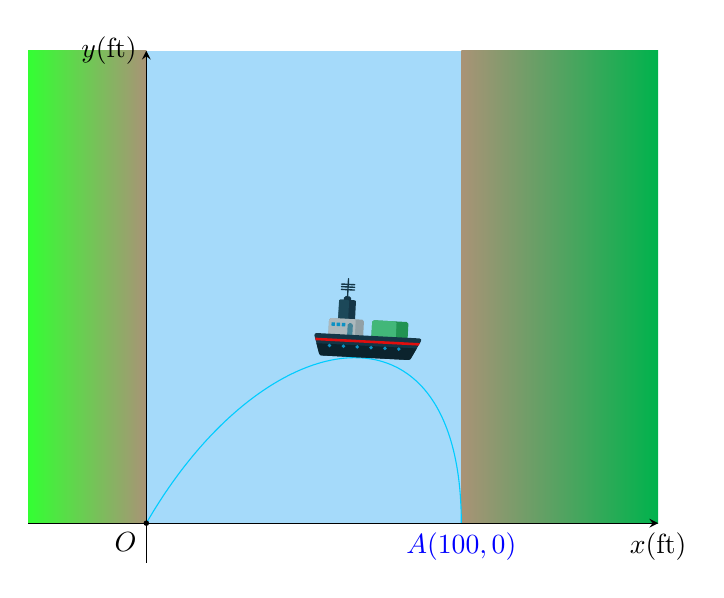
\begin{tikzpicture}[declare function={a=2; b=6;},>=stealth]
			\def\thuyen{\tikz{\path[fill={rgb,255:red,33; green,147; blue,82}]  (18.44,6.25).. controls (18.44,6.08) and (18.3,5.91)..
				(18.1,5.91) -- (11.62,5.91).. controls  (11.44,5.91) and (11.27,6.04)..
				(11.27,6.25)  -- (11.27,9.93).. controls (11.27,10.11) and (11.41,10.28)..
				(11.62,10.28) -- (18.1,10.28)..  controls (18.27,10.28) and (18.44,10.14)..
				 (18.44,9.93) -- (18.44,6.25) -- cycle;
			\path[fill={rgb,255:red,66; green,183; blue,121}] (16.09,6.25) -- (16.09,9.93).. controls (16.09,10.11) and  (15.95,10.28)..
				(15.74,10.28) -- (11.62,10.28).. controls (11.44,10.28) and (11.27,10.14).. 
				(11.27,9.93) -- (11.27,6.25)..  controls (11.27,6.08) and (11.41,5.91)..
				(11.62,5.91) -- (15.74,5.91)..  controls (15.92,5.91) and (16.09,6.04)..
				 (16.09,6.25) -- cycle;
			\path[fill={rgb,255:red,20; green,54; blue,71}] (6.29,13.55).. controls (6.29,13.48) and (6.22,13.42).. 
				(6.16,13.42)  -- (6.16,13.42).. controls (6.09,13.42) and (6.02,13.48)..
				(6.02,13.55)  -- (6.02,18.23).. controls (6.02,18.3) and (6.09,18.36)..
				(6.16,18.36) -- (6.16,18.36)..  controls (6.22,18.36) and (6.29,18.3)..
				 (6.29,18.23) -- (6.29,13.55) -- cycle;
			\path[fill={rgb,255:red,20; green,54; blue,71}] (6.87,11.5).. controls  (6.87,11.33) and (6.74,11.16)..
				(6.53,11.16) -- (5.78,11.16).. controls (5.61,11.16) and (5.44,11.3).. 
				(5.44,11.5) -- (5.44,14.41).. controls  (5.44,14.58) and (5.58,14.75)..
				(5.78,14.75) -- (6.53,14.75)..  controls (6.7,14.75) and (6.87,14.61)..
				(6.87,14.41) -- (6.87,11.5)  -- cycle;
			\path[fill={rgb,255:red,20; green,54;  blue,71}] (7.86,6.73).. controls (7.86,6.62) and (7.76,6.52)..
				(7.66,6.52) -- (4.76,6.52).. controls (4.62,6.52)  and (4.55,6.62)..
				 (4.55,6.73) -- (4.55,13.83).. controls (4.55,13.93) and (4.65,14.03)..
				(4.76,14.03) -- (7.66,14.03).. controls (7.76,14.03)  and (7.86,13.93)..
				(7.86,13.83) -- (7.86,6.73) -- cycle; 
			\path[fill={rgb,255:red,28; green,72; blue,89}] (6.5,6.73) -- (6.5,13.83).. controls (6.5,13.93) and  (6.39,14.03)..
				(6.29,14.03) --  (4.72,14.03).. controls (4.59,14.03) and (4.52,13.93)..
				(4.52,13.83)  -- (4.52,6.73).. controls (4.52,6.62) and (4.62,6.52)..
				(4.72,6.52) -- (6.29,6.52).. controls (6.43,6.49) and (6.5,6.59).. 
				 (6.5,6.73) -- cycle;
			\path[fill={rgb,255:red,146; green,160;  blue,165}] (9.6,6.66).. controls (9.6,6.49) and (9.47,6.32)..
				(9.26,6.32) -- (3.08,6.32)..  controls (2.91,6.32) and (2.74,6.45)..
				(2.74,6.66)  -- (2.74,9.93).. controls (2.74,10.11) and (2.88,10.28)..
				 (3.08,10.28) -- (9.3,10.28).. controls (9.47,10.28) and (9.64,10.14)..
				(9.64,9.93) -- (9.64,6.66) -- (9.6,6.66) -- cycle; 
			\path[fill={rgb,255:red,172; green,184; blue,188}] (3.08,10.28)..  controls (2.91,10.28) and (2.74,10.14)..
				(2.74,9.93) -- (2.74,6.73) -- (7.66,6.73).. controls  (7.83,6.73) and (8,6.86)..
				(8,7.07) -- (8,10.28) --  (3.08,10.28) -- cycle;
			\path[fill={rgb,255:red,69; green,133; blue,153}] (7.49,7.03).. controls (7.49,6.86) and  (7.35,6.69)..
				 (7.15,6.69) -- (6.8,6.69).. controls (6.63,6.69) and (6.46,6.83)..
				(6.46,7.03)  -- (6.46,9.12).. controls (6.46,9.29) and (6.6,9.46)..
				(6.8,9.46) -- (7.15,9.46).. controls  (7.32,9.46) and (7.49,9.32)..
				(7.49,9.12)  -- (7.49,7.03) -- cycle;
			\path[fill={rgb,255:red,20;  green,54; blue,71}] (21.1,7).. controls (21.03,7.1) and (20.9,7.17)..
				 (20.79,7.17) -- (0.39,7.17).. controls (0.29,7.17) and (0.15,7.1)..
				(0.08,7.03).. controls (0.01,6.93) and (-0.02,6.83).. 
				(0.01,6.69) -- (1.14,3.08)..  controls (1.17,2.91) and (1.34,2.8)..
				(1.48,2.8) -- (18.88,2.8).. controls (19.02,2.8) and (19.16,2.87).. 
				(19.23,3.01) -- (21.1,6.62).. controls (21.2,6.76) and  (21.17,6.9)..
				 (21.1,7) -- cycle;
			\path[fill={rgb,255:red,11; green,35; blue,45}] (1.14,3.08).. controls  (1.17,2.91) and (1.34,2.8)..
				(1.48,2.8)  -- (18.88,2.8).. controls (19.02,2.8) and (19.16,2.87)..
				(19.23,3.01) -- (20.35,5.16) -- (0.49,5.16) --  (1.14,3.08) -- cycle;
			\path[fill={rgb,255:red,224; green,14; blue,14}]  (0.32,5.74) -- (20.66,5.74) -- (20.93,6.25) -- (0.18,6.25) -- (0.32,5.74)-- cycle;
			\path[fill={rgb,255:red,12; green,145; blue,196}] (3.08,4.85) circle  (0.38cm);
			\path[fill={rgb,255:red,12; green,145; blue,196}]  (5.85,4.85) circle (0.38cm);
			\path[fill={rgb,255:red,12; green,145; blue,196}]  (8.58,4.85) circle (0.38cm);
			\path[fill={rgb,255:red,12; green,145; blue,196}]  (11.31,4.85) circle (0.38cm);
			\path[fill={rgb,255:red,12; green,145;  blue,196}] (14.07,4.85) circle (0.38cm);
			\path[fill={rgb,255:red,12;  green,145; blue,196}] (16.8,4.85) circle (0.38cm);
			\path[fill={rgb,255:red,12; green,145; blue,196}] (3.94,8.84).. controls  (3.94,8.81) and (3.9,8.77)..
				(3.87,8.77) -- (3.32,8.77).. controls (3.29,8.77) and (3.26,8.81).. 
				(3.26,8.84) -- (3.26,9.39).. controls (3.26,9.42) and  (3.29,9.46)..
				(3.32,9.46) -- (3.87,9.46).. controls (3.9,9.46) and  (3.94,9.42)..
				(3.94,9.39) -- (3.94,8.84) -- cycle; 
			\path[fill={rgb,255:red,12; green,145;  blue,196}] (4.96,8.84).. controls (4.96,8.81) and (4.93,8.77)..
				(4.89,8.77) -- (4.35,8.77).. controls (4.31,8.77) and  (4.28,8.81)..
				(4.28,8.84) -- (4.28,9.39).. controls  (4.28,9.42) and (4.31,9.46)..
				 (4.35,9.46) -- (4.89,9.46).. controls (4.93,9.46) and (4.96,9.42)..
				(4.96,9.39) -- (4.96,8.84) --  cycle;
			\path[fill={rgb,255:red,12; green,145;  blue,196}] (5.99,8.84).. controls (5.99,8.81) and (5.95,8.77)..
				(5.92,8.77) --  (5.37,8.77).. controls (5.34,8.77) and (5.3,8.81)..
				(5.3,8.84) -- (5.3,9.39).. controls (5.3,9.42) and (5.34,9.46).. 
				(5.37,9.46) --  (5.92,9.46).. controls (5.95,9.46) and (5.99,9.42)..
				(5.99,9.39) -- (5.99,8.84)  -- cycle;
			\path[fill={rgb,255:red,20; green,54;  blue,71}] (7.59,17.1).. controls (7.59,17.03) and (7.52,16.96)..
				(7.45,16.96) -- (4.86,16.96).. controls (4.79,16.96)  and (4.72,17.03)..
				(4.72,17.1)  -- (4.72,17.1).. controls (4.72,17.17) and (4.79,17.24)..
				(4.86,17.24) --  (7.45,17.24).. controls (7.52,17.24) and (7.59,17.17)..
				(7.59,17.1)  -- (7.59,17.1) -- cycle;
			\path[fill={rgb,255:red,20; green,54;  blue,71}] (7.59,16.59).. controls (7.59,16.52) and (7.52,16.45)..
				(7.45,16.45)  -- (4.86,16.45).. controls (4.79,16.45) and (4.72,16.52)..
				(4.72,16.59) -- (4.72,16.59)..  controls (4.72,16.66) and (4.79,16.73)..
				(4.86,16.73) -- (7.45,16.73).. controls (7.52,16.69) and (7.59,16.66).. 
				(7.59,16.59) -- (7.59,16.59) --  cycle;
			\path[fill={rgb,255:red,20; green,54; blue,71}] (7.59,16.04)..  controls (7.59,15.97) and (7.52,15.91)..
				(7.45,15.91)  -- (4.86,15.91).. controls (4.79,15.91) and (4.72,15.97)..
				(4.72,16.04) -- (4.72,16.04)..  controls (4.72,16.11) and (4.79,16.18)..
				(4.86,16.18) -- (7.45,16.18).. controls  (7.52,16.18) and (7.59,16.11)..
				 (7.59,16.04) -- (7.59,16.04) -- cycle;}}
			\definecolor{ca99376}{RGB}{169,147,118} 
			 \definecolor{ca5dafa}{RGB}{165,218,250}
			\fill[ca5dafa] (0,0)  rectangle (4,b);
			\path[right color=ca99376,left  color=green!80!white] (0,0) rectangle (-1.5,b);
			\path[left color=ca99376,right color=green!70!blue] (4,0)  rectangle +(2.5,b);
			\draw[blue!20!cyan]  (0,0).. controls +(60:3) and +(90:3).. (4,0) node[below,blue]{$A (100,0)$}
				 node[pos=0.55,rotate=-3,anchor=south,inner sep=0pt] {\resizebox{!}{1cm}{\thuyen}};
			\draw[->] (-1.5,0)--(6.5,0)  node[below]{$x$(ft)};
			\draw[->]  (0,-0.5)--(0,6) node[left]{$y$(ft)};
			\fill  (0,0) circle (1pt) node[below left]{$O$};
		\end{tikzpicture}
	\end{center}
	Tìm độ lệch bắc lớn nhất mà thuyền đạt được trong  suốt hành trình.
	 \shortans{76,6}
	\loigiai{ 
		Đặt $u=\dfrac{1000-x}{1000}$  thì $0\leq u \leq 1$ và $x=1000(1-u)$.\\
		Khi đó $y(u)=500\left(u^{3/ 4}-u^{5/ 4}\right)$.\\ 
		Tính đạo hàm theo $u$ ta được $y'(u)=500\left(\dfrac{3}{4}  u^{-1/ 4}-\dfrac{5}{4} u^{1/ 4}\right)=500\cdot \dfrac{1}{4} u^{-1/ 4}\left(3-5u\right)$.\\
		Vì $u^{-1/ 4} > 0$ trên $(0{,}1]$, ta chỉ cần giải  $3-5u=0\Rightarrow u=\dfrac{3}{5}=0{,}6$.\\
		Lập bảng biến thiên ta  có
		\begin{center}
			
\begin{tikzpicture}[font=\normalsize]
				\tkzTabInit[lgt=1.2,espcl=2.5,deltacl=0.8] 
					{$x$  /0.75,$y'(u)$/0.75,$y (u)$/2}
					{$  0 $,$ 0{,}6 $,$ 20 $}
				\tkzTabLine{,+,0,-,} 
				\tkzTabVar{-/$0$,+/${y (0{,}6)}$,-/${y (20)}$} 
			\end{tikzpicture}
		\end{center}
		Suy ra $y(u)$  đạt điểm cực đại tại $u=0{,}6$.\\
		Khi đó $x=1000(1-u)=1000\cdot 0{,}4=400$ và độ lệch bắc lớn nhất là $$y_{\text{ CĐ}}=500\left((0{,}6)^{3/ 4}-(0{,}6)^{5/ 4}\right)  \approx 500(0{,}6817-0{,}5286) \approx 76{,}6.$$
		Do đó trong suốt hành trình, con thuyền bị dòng nước đẩy  lệch về phía bắc cực đại khoảng $76{,}6$ (đơn vị chiều dài) khi nó đã đi được $x=400$ (đơn vị tương ứng) về phía đông.
	} 
\end{bt}

% nguồn: Phan2_Lop_12_Dai_so_Chuong_1
\begin{bt}%[2D1V2-7]%[ma:7b9935f7]
	Một khu vực trồng hoa được xây dựng trong khu du lịch sinh thái. Trong mô hình minh họa (như hình vẽ bên), nó được giới hạn bởi các trục tọa độ và đồ thị $(C)$ của một hàm số bậc ba. Biết rằng đồ thị $(C)$ đi qua các điểm $A(0; 8), B(2; 5,4), K(5; 6,75)$ và $H(8; 0)$. Trong khu du lịch sinh thái  có một con đường chạy dọc theo đường thẳng $d: y=-\dfrac{13}{9} x+\dfrac{169}{9}$. Tìm hoành độ của điểm $M$ thuộc $(C)$ sao cho khoảng cách từ $M$ đến $d$ là nhỏ nhất (làm tròn kết quả đến hàng phần trăm).
	\begin{center}
		\begin{tikzpicture}[line join = round,line cap=round,>=stealth,font=\footnotesize,scale=0.5]
			 \def\f (\x){(-0.1*(\x)^3+1.05*(\x)^2-3*(\x)+8)}
			\draw[->]  (-0.5,0)--(0,0) node[below
				 left]{$O$}--(14,0)
				 node[above]{$x$};
			\draw[->] (0,-0.5)--(0,11) 
				 node[left]{$y$};
			 \fill[pattern=crosshatch dots,smooth] (0,0) --
				plot[domain=0:8] (\x,{\f (\x)}) 
				-- (8,0)  -- cycle;
			\draw[smooth,red,line width=1] 
				 plot[domain=0:8]
				(\x,{\f  (\x)});
			\draw (2,0) node[below]{$2$} 
				 (13,0) node[below]{$13$}
				(8,0) node[below]{$8$} 
				(8,0) node[above right]{$H$} 
				 (0,8) node[right]{$A$}
				 (6,10) node[right]{$d$}
				 (5,0) node[below]{$5$}
				(0,8) node[left]{$8$} 
				(0,6.75)  node[left]{$6,75$}
				 (0,5.4) node[left]{$5,4$};
			\draw[line  width=1pt]((4.6,11)--(13,0);
			\draw[dashed] (5,0)--(5,6.75) node[above]{$K$}--(0,6.75) 
				(2,0)--(2,5.4)  node[above]{$B$}--(0,5.4);
		\end{tikzpicture}
	\end{center}
	 \shortans{6,16}
	 \loigiai{
		Đồ thị $(C)$ của một hàm số  bậc ba có dạng: $f(x)=a x^3+b x^2+c x+d(a \neq 0)$.
		Vì  đồ thị $(C)$ đi qua các điểm $A(0; 8), B(2; 5,4), K(5; 6,75)$ và $H(8; 0)$ nên ta có:
		$\left\{\begin{array}{l}d=8 \\ 8 a+4 b+2 c+d=5,4 \\ 125 a+25 b+5 c+d=6,75 \\ 512 a+64 b+8 c+d=0
	\end{array} \Leftrightarrow\left\{\begin{array}{l}a=-\dfrac{1}{10} \\ b=\dfrac{21}{20} \\ c=-3 \\ d=8
	\end{array}\right.\right.$.
	Suy ra $f(x)=-\dfrac{1}{10} x^3+\dfrac{21}{20} x^2-3 x+8$. 
	Điểm $M$ thuộc $(C)$ sao cho khoảng cách từ $M$ đến $d$ là nhỏ nhất khi và chỉ khi tiếp tuyến của $(C)$ tại $M$  song song với $d\left(x_M>5\right)$.
	 Ta có: $f'(x)=-\dfrac{3}{10} x^2+\dfrac{21}{10} x-3$.
	Đường thẳng $d$  có hệ số góc $k=-\dfrac{13}{9}$.
	Suy ra: $-\dfrac{3}{10} x^2+\dfrac{21}{10} x-3=-\dfrac{13}{9} \Leftrightarrow\left[\begin{array}{l}x=6,16 \\ x=0,84<5
	\end{array}\right.$.
	Do $x_M>5$ nên $x_M=6,16$ thỏa  mãn.
	 }
	\end{bt}

% nguồn: Phan2_Lop_12_Dai_so_Chuong_1
\begin{bt}%[2D1V2-7]%[ma:5ad548bc]
		Một bể ban đầu chứa $10$ gal dung dịch muối với $2$ lb muối. Dung dịch vào có nồng độ $1{,}5$ lb/gal chảy vào với tốc độ $3$ gal/phút, và hỗn hợp trong bể chảy ra với tốc độ $4$ gal/phút. Người ta cho biết lượng muối  trong bể sau $t$ phút là $x$ (pound), với
		$$ 
		x=f(t)=1{,}5(10-t)-0{,}0013(10-t)^4, \quad 0 \leq t \leq  10.
		$$ 
		Hỏi lượng muối tối đa có thể có trong  bể tại một thời điểm nào đó là bao nhiêu lb? (\textit{làm tròn kết quả đến hàng phần trăm}).
		\begin{center}
		 \definecolor{columbiablue}{rgb}{0.61, 0.87, 1.0}
		 \definecolor{cyan(process)}{rgb}{0.0, 0.72, 0.92}
			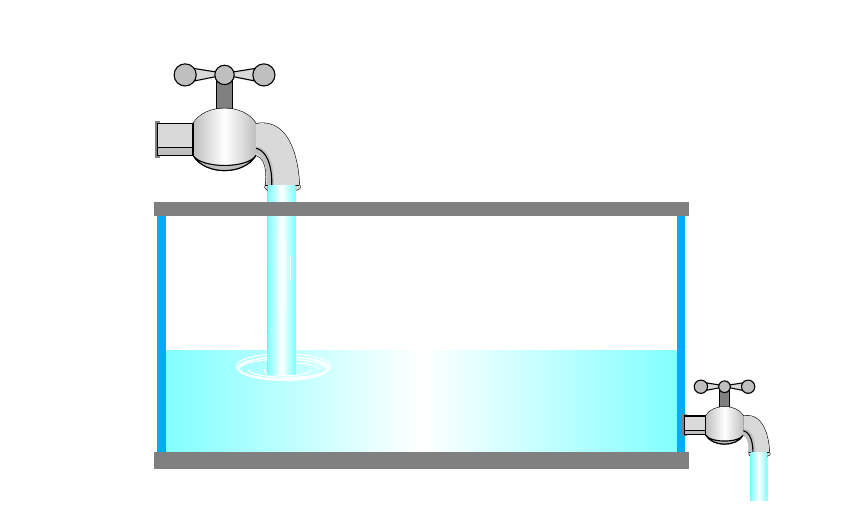
\begin{tikzpicture}
				\clip  (-5,-3) rectangle (5,3);
				\begin{pgfinterruptboundingbox}
					\tikzset{voi/.pic={ 
					 \draw[fill=gray!30](-2.5,2.42)--(-2,2.5)--(-2,2.3)--(-2.5,2.4)--(-3,2.3)--(-3,2.5)--cycle;
					\draw[fill=gray] (-2.4,2.4)--(-2.6,2.4)--(-2.6,1.9)--(-2.4,1.9)--cycle; 
					\draw[fill=gray!50] (-2.5,2.4)  circle (3.5pt);
					\draw[fill=gray!50] (-2,2.4) circle  (4pt);
					\draw[fill=gray!50]  (-3,2.4) circle (4pt);
					\def\E{ 
						(-2.9,1.78) 
						 ..controls +(60:.3) and +(120:0.3)..(-2.1,1.78)--(-2.1,1.38)
						..controls  +(-120:.3) and +(-60:0.3)..(-2.9,1.38);}
					\draw\E; 
					\fill[left  color=gray!50,right color=gray!50,middle color=white]\E;
					 \def\E{
						 (-2.1,1.38)
						 ..controls +(-15:.18) and +(90:0)..(-1.98,1)
						..controls +(-120:.1) and  +(0:0)..(-1.8,.92)
						..controls +(0:.35)  and +(-120:0)..(-1.55,1)
						..controls +(90:0)  and +(10:.55)..(-2.1,1.78);}
					\def\F{ 
						 (-2.1,1.38)
						..controls +(-120:.3) and  +(-60:0.3)..(-2.9,1.38)
						..controls +(-60:.2) and +(-120:0.2)..(-2.1,1.38);} 
					\fill[gray!50] \F; 
					\draw\F; 
					\draw\E; 
					 \fill[gray!30] \E;
					\draw[color=gray!50,line  width=2.5](-2.1,1.45)
						..controls +(-15:.22)  and +(90:0)..(-1.92,1);
					 \draw[color=black](-1.98,1)--(-1.55,1);
					 \draw (-2.1,1.47)
						..controls +(-15:.23) and +(90:0)..(-1.9,1); 
					\draw[color=gray,line width=1.7]  (-3.35,1.82)--(-3.35,1.35);
					\draw[fill=gray!30]  (-3.35,1.78)--(-2.9,1.78)--(-2.9,1.38)--(-3.35,1.38)--cycle;
					 \draw[fill=gray!50] (-3.35,1.48)--(-2.9,1.48)--(-2.9,1.38)--(-3.35,1.38)--cycle;
					 \fill[left color=cyan!50,right color=cyan!50,middle color=white] (-1.95,1)--(-1.6,1)--(-1.6,-1.4)--(-1.95,-1.4)--(-1.95,1);
						 }}
					\tikzset{ho_nuoc/.pic={ 
					\fill[left color=cyan!50,right  color=cyan!50,middle color=white](-3.3,-2.5)--(3.3,-2.5)--(3.3,-1.1)--(-3.3,-1.1);
					 \draw[color=cyan,line width=3](-3.3,-2.5)--(-3.3,.7)
						(3.3,-2.5)--(3.3,.7); 
					\draw[color=white] (-1.15,-1.3) arc (0:360:.6 cm and 0.16cm)--cycle; 
					\draw[color=white] (-1.17,-1.32) arc (0:360:.58 cm and  0.14cm)--cycle;
					\draw[color=white]  (-1.19,-1.33) arc (0:360:.56 cm and 0.15cm)--cycle;
					\draw[color=white] (-1.2,-1.34) arc (0:360:.56 cm and 0.13cm)--cycle; 
					\draw[color=white] (-2.2,-1.34)  arc (-180:0:.5 cm and 0.1cm);
					\draw[color=white]  (-2,-1.34) arc (-180:0:.3 cm and 0.08cm);
					 \draw[color=white] (-1.3,-1.34) arc (0:180:.3 cm and 0.08cm);
					\fill[left color=cyan!50,right  color=cyan!50,middle color=white]
						(-1.95,1)--(-1.6,1)--(-1.6,-1.4)--(-1.95,-1.4)--(-1.95,1); 
					\draw[color=white]  (-1.8,.5)--(-1.8,-.7)
						 (-1.66,.1)--(-1.66,-.2)
						 (-1.72,.3)--(-1.72,-.6)
						 (-1.9,0)--(-1.9,-.9);
					\draw[color=gray,line  width=5](-3.4,.7)--(3.4,.7);
					\draw[color=gray,line  width=6](-3.4,-2.5)--(3.4,-2.5);
						 }}
					 \path (0,0) pic[scale=1]{voi};
					 \path (0,0) pic[scale=1]{ho_nuoc};
					\path (5.35,-3) pic[scale=0.6]{voi}; 
				\end{pgfinterruptboundingbox}
			\end{tikzpicture}
		\end{center}
	 \shortans{7,43}
	 \loigiai{
		Ta có công thức  lượng muối $x$ (pound) trong bể sau $t$ phút là
		 $$
		x(t)=1{,}5(10-t)-0{,}0013(10-t)^4; \quad 0 \leq t  \leq 10.
		 $$
		 Đặt $u=10-t$. Khi $t$ chạy từ $0$ đến $10$ thì $u$ chạy từ $10$ xuống $0$.\\
		Khi đó $x(u)=1{,}5u-0{,}0013u^4$; $ 0\leq u \leq  10$.\\
		Tính đạo hàm theo $u$ ta được $x'(u)=1{,}5-0{,}0013\cdot 4u^3=1{,}5-0{,}0052u^3$.\\ 
		Xét $1{,}5-0{,}0052u^3=0\Rightarrow u^3=\dfrac{1{,}5}{0{,}0052} \approx 288{,}46\Rightarrow u = \sqrt[3]{\dfrac{1{,}5}{0{,}0052}} \approx 6{,}62$.\\ 
		 Lập bảng biến thiên ta được
		\begin{center}
			
\begin{tikzpicture}[font=\normalsize]
				 \tkzTabInit[lgt=1.2,espcl=3,deltacl=0.7]
					 {$u$ /0.75,$x'(u)$/0.75,$x (u)$/2.5}
					{$ 0 $,$\sqrt[3]{\tfrac{1{,}5}{0{,}0052}}$,$  10 $}
				\tkzTabLine{,+,0,-,} 
				\tkzTabVar{-/$0$,+/$1{,}125\cdot\sqrt[3]{\tfrac{1,5}{0,0052}}$,-/$2$} 
			\end{tikzpicture}
		\end{center}
		Suy ra hàm số đạt cực đại tại $u=\sqrt[3]{\dfrac{1{,}5}{0{,}0052}} \approx 6{,}62$ với giá  trị cực đại
		$$x_{\text{ CĐ}}=1{,}5\cdot 6{,}62-0{,}0013(6{,}62)^4\approx  9{,}93-2{,}50\approx 7{,}43 \,\mathrm{lb}.$$
		Lượng muối trong bể đạt tối đa  khoảng $7{,}43$ lb tại thời điểm $t \approx 3{,}38$ phút kể từ lúc bắt đầu.
	 }
\end{bt}

% nguồn: Phan2_Lop_12_Dai_so_Chuong_1
\begin{bt}%[2D1V2-7]%[ma:195835f6]
	Khi chất thải hữu cơ được đổ vào một cái ao, quá  trình ôxy hóa xảy ra sẽ làm giảm hàm lượng ôxy trong nước. Tuy nhiên, theo thời gian, tự nhiên sẽ phục hồi lại mức ôxy về giá trị bình thường. Trong đồ thị kèm theo, $P(t)$ cho biết phần trăm hàm lượng ôxy (so với mức bình thường) sau $t$ ngày kể từ khi chất thải được đổ vào ao.\\
	Giả  sử hàm số cho hàm lượng ôxy là $P(t)=100\cdot\dfrac{t^2+10t+100}{t^2+20t+100}$ ($\%$ mức bình thường), $t \geq 0$.
	\begin{center}
		\begin{tikzpicture}[line join = round,line cap = round,>=stealth,font=\footnotesize,yscale=1/35,xscale=1/25]
			\def\xmin{-10}  \def\xmax{100}
			 \def\ymin{-10} \def\ymax{130}
			\def\f  (#1){100*(((#1)^2+10*(#1)+100)/((#1)^2+20*(#1)+100))}
			\def\xp{10} 
			\pgfmathsetmacro{\yp}{\f  (\xp)}
			\foreach \x in {} \draw (\x,2pt)--(\x,-2pt)  node [below] {$\x$};
			 \draw[-stealth] (\xmin,0)--(\xmax,0) node[below]{$t\,\left(\text{ngày}\right)$};
			\foreach \y in  {75,100} \draw (2,\y)--(-2,\y) node [left] {$\y$};
			 \draw[-stealth] (0,\ymin)--(0,\ymax) node[left]{$y\,\left(\%\right)$};
			\filldraw (0,0) node[below left]{$O$}  circle (1.5pt);
			 \clip (\xmin,\ymin) rectangle (\xmax,\ymax);
			 \draw[samples=100,domain=0:100,smooth] plot (\x,{\f (\x)});
			\draw[samples=100,domain=0:100,smooth,dashed] plot (\x,{100}); 
			\fill  (\xp,\yp) node[below]{$P$} circle (1.5);
		\end{tikzpicture}
	\end{center}
	Khi đó tọa độ của điểm $P(a;b)$ trên đồ  thị là điểm cực trị của đồ thị hàm số $P(t)$. Tính $a+b$? \shortans{85}
	\loigiai{ 
		Ta  có: $P'(t)=\dfrac{(2t+10)\left(t^2+20t+100\right)-(2t+20)\left(t^2+10t+100\right)}{\left(t^2+20t+100\right)^2}$.\\
		Khi đó \allowdisplaybreaks 
		\begin{eqnarray*}
			 &&P'(t)=0\\
			 &\Leftrightarrow&(2t+10)\left(t^2+20t+100\right)-(2t+20)\left(t^2+10t+100\right)=0\\
			 &\Rightarrow& 10t^2-1000=0\\
			 &\Rightarrow& t^2=100\\
			&\Rightarrow& t=10 \quad (t  \geqslant 0).
		\end{eqnarray*}
		Lập bảng biến thiên 
		\begin{center}
			
\begin{tikzpicture}
				\tkzTabInit[nocadre=true,lgt=1.5,espcl=3,deltacl=1] {$x$ /1.2,$P’(x)$ /1.2,$P  (x)$/2.5}{$0$,$10$,$+\infty$}
				\tkzTabLine{,-,0,+,} 
				 \tkzTabVar{+/$100$,-/$75$,+/$100$}
			\end{tikzpicture}
		\end{center}
		Ta có  $t=10$ là điểm cực tiểu của hàm số.\\
		Thay $t=10$ vào $P(t):  P(10)=100\dfrac{10^2+10\cdot 10+100}{10^2+20\cdot 10+100}=100\dfrac{100+100+100}{100+200+100}=100\dfrac{300}{400}=75$.\\
		Vậy điểm  $P$ có tọa độ $(10; 75)$
	} 
\end{bt}

% nguồn: Phan2_Lop_12_Dai_so_Chuong_1
\begin{bt}%[2D1V2-7]%[ma:2acb8871]
	Trong lớp học, màn hình tivi hình chữ nhật có chiều cao $1m$ được đặt ở  độ cao $1.2m$ so với tầm mắt của học sinh (tính từ đầu mép dưới của màn hình). Để nhìn rõ nhất phải xác định vị trí ngồi sao cho góc nhìn lớn nhất ($\widehat{BOC}$ là góc nhìn).
	\begin{center}
		\begin{tikzpicture}[scale=1.2]
			 \path
				(0,0)  coordinate (O)
				(-3,0) coordinate (A) 
				(-3,1.5) coordinate  (B)
				(-3,2.5) coordinate  (C);
			 \draw (O) node[above right]{\text{ \footnotesize Vị trí mắt}}--(B)--node[left]{\text{ \footnotesize Tivi}} node[right]{$ 1 $}
				 (C)--cycle;
			\draw[dashed]  ($(A)-(2,0)$)--($(O)+(2,0)$)
				(A)--node[right]{$ 1,2  $}
				(B); 
			\draw  pic[draw,angle radius=1cm]{angle=C--O--B};
			\draw pic[draw,angle radius=0.3cm]{right angle=O--A--B}; 
			 \foreach \i/\g in {O/-40,B/240,C/120,A/-90}{\fill (\i) circle (1pt) node[shift={(\g:10pt)}]{$\i$};}
		\end{tikzpicture}
	\end{center}
	Nếu xét những học sinh ngồi nhìn thẳng màn hình thì học sinh ngồi bàn thứ mấy nhìn được rõ  nhất, biết bàn đầu tiên cách tivi $1.2m$ và mỗi bàn kế tiếp nhau cách nhau $0.4m$.
	 \shortans{2}
	\loigiai{ 
		Đặt  $OA=x$, ta có $OB=\sqrt{x^2+1.44}$, $OC=\sqrt{x^2+4.84}$\\
		Ta có: $\cos{\widehat{BOC}} = \dfrac{OB^2+OC^2-BC^2}{2. OB.  OC} = \dfrac{x^2+2.64}{\sqrt{x^2+1.44}.\sqrt{x^2+4.84}}$\\
		Đặt $t=x^2, t>0$. Xét  $f(t) = \dfrac{t+2.64}{\sqrt{t+1.44}.\sqrt{t+4.84}} = \dfrac{t+2.64}{\sqrt{t^2+6.28t+6.9696}}$\\
		Ta  có: $f'(t) = \dfrac{0.5t-1.32}{(\sqrt{t^2+6.28t+6.9696})^3}$\\
		Khi  đó: $f'(t)=0 \Leftrightarrow t=2.64$
	} 
\end{bt}

% nguồn: Phan2_Lop_12_Dai_so_Chuong_1
\begin{bt}%[2D1V2-7]%[ma:939181a5]
	Định mức cầu mỗi tháng của đồng hồ đeo tay Peget phụ thuộc vào giá đơn vị $p$ theo phương trình cầu $p=\dfrac{50}{0{,}01x^2+1}$, $0\leq x \leq 20$ trong đó $p$ tính bằng đô la và $x$ tính bằng nghìn chiếc. Hỏi nhà sản xuất phải bán bao nhiêu nghìn chiếc để doanh thu $R=p x$ đạt cực  đại?
	\shortans{10} 
	\loigiai{ 
		Doanh thu  $R(x)$ là $R(x)=p(x) x=\dfrac{50x}{0{,}01x^2+1}$.
		 Tính đạo hàm $R'(x)$
		\begin{eqnarray*}
			R'(x)=\dfrac{\left(0{,}01 x^2+1\right) \cdot 50-50 x \cdot(0{,}02 x)}{\left(0{,}01 x^2+1\right)^2}=\dfrac{50\left(0{,}01 x^2+1-0{,}02 x^2\right)}{\left(0{,}01  x^2+1\right)^2}=\dfrac{50\left(1-0{,}01 x^2\right)}{\left(0{,}01 x^2+1\right)^2}; 0 \leq x \leq 20.
		\end{eqnarray*}
		 Giải $R'(x)=0$ ta có $1-0{,}01x^2=0\Rightarrow x^2=100\Rightarrow x=10$.\\
		 Ta có bảng biến thiên
		\begin{center}
			
\begin{tikzpicture}[font=\normalsize]
				 \tkzTabInit[lgt=1.2,espcl=2.5,deltacl=0.5]
					{$x$ /0.75,$R'(x)$/0.75,$R  (x)$/2}
					{$  0 $,$ 10 $,$ 20 $}
				\tkzTabLine{,+,0,-,} 
				 \tkzTabVar{-/$0$,+/$250$,-/$200$}
			\end{tikzpicture}
		\end{center}
		Suy ra được  hàm số đạt cực đại tại $x=10$.\\
		Khi đó  giá trị cực đại là $R(10)=250$.
	} 
\end{bt}

% nguồn: Phan2_Lop_12_Dai_so_Chuong_1
\begin{bt}%[2D1V2-7]%[ma:a412dc4a]
	Một bồn hình trụ cao $h$ chứa nước. Theo định luật  Torricelli, vận tốc tia nước chảy qua lỗ ở độ sâu $x$ so với mặt nước là $V=\sqrt{2g x}$. Người ta cho rằng tầm xa $R$ (feet) của tia nước được cho bởi $R=2\sqrt{x(h-x)}$.
	Biết lỗ phun nên đặt ở độ cao $x=K\cdot h$, ($K\in \mathbb{R}$)  so với mặt bồn thì tầm xa $R$ đạt cực đại. Tìm $K$.
	\begin{center}
		\begin{tikzpicture}
			\tikzset{declare function={theta=69;  r=2; h=6;},samples=150,smooth}
			\tdplotsetmaincoords{theta}0 
			\begin{scope}[tdplot_main_coords]
				\draw[dash pattern=on 2pt off  1.5pt] plot[domain=0:180]
					({r*cos (\x)},{r*sin  (\x)},0) coordinate (A);
				\path (0,0,0)  coordinate (O)
					(0,0,h) coordinate (O') 
					($(A)+(0,0,h)$) coordinate  (B);
				\fill[blue!50!white]  (A)--(B)--($(O')!-1!(B)$)--($(O)!-1!(A)$)--(A);
				 \draw[dash pattern=on 2pt off 1.5pt] plot[domain=0:180]
					({r*cos  (\x)},{r*sin (\x)},0);
				 \draw plot[domain=180:360]
					 ({r*cos (\x)},{r*sin (\x)},0);
				\fill[blue!50!white] plot[domain=180:360] 
					({r*cos (\x)},{r*sin (\x)},0); 
				\draw[white]  plot[domain=180:360]
					 ({r*cos (\x)},{r*sin (\x)},h/3);
				\draw[white]  plot[domain=180:360]
					 ({r*cos (\x)},{r*sin (\x)},2*h/3);
				 \fill[blue!50!white] plot[domain=0:180]
					({r*cos (\x)},{r*sin  (\x)},h);
				\draw  (A)--+(0,0,h)
					 (-r,0,0)--+(0,0,h)
					plot[domain=0:360]({r*cos  (\x)},{r*sin (\x)},h);
			\end{scope}
			\path ($(O')!-1!(B)$) coordinate  (B')
				($(O)!-1!(A)$) coordinate  (A')
				($(O)!-5/2!(A)$) coordinate (D) 
				($(B')!1/5!(A')$) coordinate  (C);
			\draw (B')--  (A');
			 \draw[>=stealth,|<->|] ($(B')+(0:7pt)$)--($(C)+(0:7pt)$) node[inner sep=3pt,pos=0.5,right]{$x$};
			\draw[>=stealth,|<->|] ($(A')+(-90:7pt)$)--($(D)+(-90:7pt)$)  node[fill=white,inner sep=3pt,pos=0.5,below]{$R$};
			\path  (A)--(B)
				(B)++(180:7pt)  coordinate (xt)
				($(A)-(B)+(xt)$) coordinate  (yt);
			\draw[>=stealth,|<->|] (xt)--(yt) node[fill=white,inner sep=3pt,pos=0.5,left]{$h$}; 
			\tikzset{declare function={f  (\x)=-1/2*(\x)^2+2*(\x)+5/2;}}
			\begin{scope}
				\draw[samples=100,line width=0.9mm,blue]  plot[domain=2:5] (\x,{f (\x)});
			\end{scope}
		\end{tikzpicture}
	\end{center}
	 \shortans{0,5}
	\loigiai{ 
		Thay vì trực tiếp  giá trị lớn nhất $R(x)$, ta có thể tìm giá trị lớn nhất $R^2(x)$. Ta có
		$$ 
		 R^2(x)=4 x(h-x)=4\left(h x-x^2\right).
		 $$
		Tính đạo hàm  $\left(R^2(x)\right)'=4(h-2x)$.\\
		 Giải $\left(R^2(x)\right)'=0$ ta được $h-2x=0\Rightarrow x=\dfrac{h}{2}$.\\
		Ta có bảng  biến thiên
		\begin{center}
			
\begin{tikzpicture}[font=\normalsize]
				 \tkzTabInit[lgt=1.5,espcl=2.5,deltacl=0.5]
					{$x$ /0.75,$R^2  (x)'$/0.75,$R^2 (x)$/2}
					 {$ 0 $,$ \tfrac{h}{2} $,$ h $}
				\tkzTabLine{,+,0,-,} 
				 \tkzTabVar{-/$0$,+/$h^2$,-/$0$}
			\end{tikzpicture}
		\end{center}
		Từ  bảng biến thiên ta có $x=\dfrac{h}{2}$ là điểm cực đại.\\
		Vậy lỗ phun nên  đặt ở độ cao $x=\dfrac{h}{2}$ để tầm xa $R$ của tia nước đạt tối đa.
	} 
\end{bt}

% nguồn: Phan2_Lop_12_Dai_so_Chuong_1
\begin{bt}%[2D1V2-7]%[ma:b888b4f3]
	Hằng ngày, mực nước của hồ thủy điện ở miền Trung lên và xuống theo lượng nước mưa và các suối nước đổ về hồ. 
	Tính từ thời điểm $8$ giờ sáng, độ sâu của mực nước trong hồ (tính theo mét) thay đổi theo thời gian $t$ (giờ) trong ngày, được mô tả bởi công thức: $h(t) = -\dfrac{1}{3}t^3 +  5t^2 + 24t\,(t > 0)$.
	Biết rằng phải thông báo cho các hộ dân di dời trước khi  xả nước theo quy định là trước $5$ giờ.
	Hỏi cần thông báo cho hộ dân di dời sau bao~nhiêu giờ? Biết rằng  mực nước trong hồ phải lên cao nhất mới xả nước.
	\shortans{7} 
	\loigiai{$h'(t) = 0 \Leftrightarrow  -t^2 + 10t + 24 = 0\Leftrightarrow t=12$.
		 Xét dấu của $h'(t)$
		\begin{center}
			
\begin{tikzpicture}
				 \tkzTabInit[nocadre,lgt=1.5,espcl=4.5]
					{$t$/1,$h'(t)$/1,$h (t)$/2} 
					 {$0$,$12$,$+\infty$}
				\tkzTabLine{,+,0,-,} 
				 \tkzTabVar{-/$ $,+/$h_{\text{ max}}$,-/$ $/}
			\end{tikzpicture}
		\end{center}
		Để mực nước dâng lên tới điểm cao nhất, cần mất $12$ giờ.  Sau $20$ giờ, mực nước đầy. Do đó, cần thông báo cho người dân di dời sau $7$ giờ.
	} 
\end{bt}

% nguồn: Phan2_Lop_12_Dai_so_Chuong_1
\begin{bt}%[2D1V2-7]%[ma:82a38056]
	Sau  khi kinh tế suy giảm, giá thuê văn phòng cao ngất ngưởng cuối thập niên $1990$ bắt đầu hạ nhiệt. Hàm $R(t)$ cho giá thuê (USD/ft$^2$) của văn phòng hạng A ở khu Back Bay và Financial District (Boston) từ đầu $1997$ ($t=0$) đến đầu $2002$ ($t=5$) là
	 $$
	R(t)=-0{,}711 t^3+3{,}76 t^2+0{,}2 t+36{,}5; \quad 0 \leq t \leq 5. 
	$$ 
	Hỏi giá thuê cao nhất trong giai đoạn này là bao nhiêu? (\textit{làm tròn  kết quả đến hàng phần mười}).
	\shortans{52,8} 
	\loigiai{ 
		Tính đạo hàm 
		$$R'(t)=\left(-0{,}711t^3+3{,}76t^2+0{,}2t+36{,}5\right)^{\prime}=-2{,}133t^2+7{,}52t+0{,}2.$$ 
		Giải $R'(t)=0$ ta  có $-2{,}133t^2+7{,}52t+0{,}2=0$
		Áp dụng công thức nghiệm ta được 
		 $$
		t=\dfrac{-7{,}52 \pm \sqrt{7{,}52^2-4(-2{,}133)(0{,}2)}}{2(-2{,}133)} =\dfrac{3760}{2133} \pm \dfrac{2  \sqrt{3555730}}{2133}.
		 $$
		Hai  nghiệm thu được $t_1= \dfrac{3760}{2133} - \dfrac{2 \sqrt{3555730}}{2133} \approx-0{,}03$ (loại), $t_2= \dfrac{3760}{2133} + \dfrac{2 \sqrt{3555730}}{2133} \approx 3{,}55$.\\
		Ta lập  được bảng biến thiên
		\begin{center}
			
\begin{tikzpicture}[font=\normalsize]
				\tkzTabInit[lgt=1.2,espcl=5,deltacl=1] 
					{$t$ /0.75,$R'(t)$/0.75,$R (t)$/2} 
					{$ 0 $,$\tfrac{3760}{2133}  + \tfrac{2 \sqrt{3555730}}{2133}$,$ 5 $}
				 \tkzTabLine{,+,0,-,}
				 \tkzTabVar{-/$0{,}2$,+/$52{,}8$,-/$-15{,}525$}
			\end{tikzpicture}
		\end{center}
		Từ bảng biến thiên ta suy ra được hàm số đạt cực đại tại $t \approx 3{,}55$.\\ 
		Hay giá thuê  cao nhất là $R(3{,}55) \approx 52{,}8$ USD/ft$^2$
	 }
\end{bt}


%%%%%%%%%%%%%%%% TỰ LUẬN %%%%%%%%%%%%%%%%

% nguồn: Phan2_Lop_12_Dai_so_Chuong_1
\begin{bt}%[2D1V2-7]%[ma:f5527ce0]
	\immini{Một vật chuyển động với vận tốc $ v~( \text{ km/h})$ phụ thuộc vào thời gian $ t~( \text{ h})$ có đồ thị của hàm số dạng hàm bậc ba như hình bên. Biết rằng tại thời điểm $t_1=1~\text{ h}$ vật có vận tốc $v_1=4~\text{ km/h}$ và tại thời điểm $t_2=2~\text{ h}$ vật có vận tốc $v_2=1~\text{ km/h}$. Tính vận tốc của vật tại thời điểm $ t=3~\text{ h}$.}{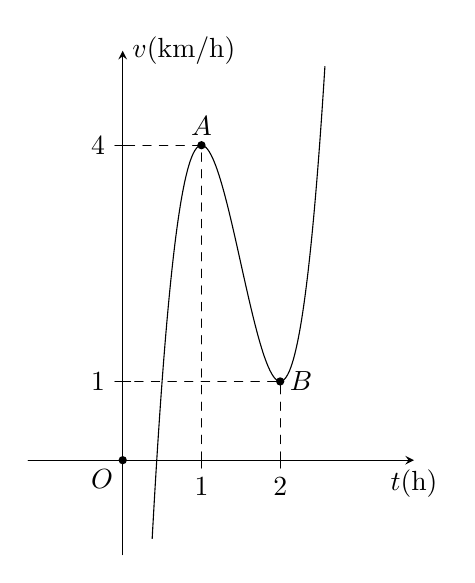
\begin{tikzpicture}[scale=1,line join=round,line cap=round,>=stealth]
		\tikzset{ethicknode/.style={scale=1}} 
		 \def\xmin{-1}\def\xmax{3.5}\def\ymin{-1}\def\ymax{5}
		\draw[->] (\xmin-0.2,0)--(\xmax+0.2,0)  node[below]{$t$(h)};
		 \draw[->] (0,\ymin-0.2)--(0,\ymax+0.2) node[right]{$v$(km/h)};
		 \draw (0,0) node[below left]{$O$};
		\foreach  \x in {1,2}\draw (\x,0.1)--(\x,-0.1) node[below]{$\x$};
		\foreach \y  in {1,4}\draw (0.1,\y)--(-0.1,\y) node[left]{$\y$};
		\clip  (\xmin,\ymin) rectangle (\xmax,\ymax);
		\draw[smooth,samples=200,domain=\xmin:\xmax] plot  (\x,{6*((\x)^3)+-27*((\x)^2)+36*(\x)+-11});
		\draw[dashed] (1,0)--(1,4)--(0,4); \fill (1,4) circle (1.5pt); \fill (0,0)  circle (1.5pt);
		\draw[dashed] (2,0)--(2,1)--(0,1); \fill (2,1) circle (1.5pt); 
		\coordinate [label=above:$A$](A) at (1,4); 
		\coordinate [label=right:$B$](B)  at (2,1);
	\end{tikzpicture}
	} 
	\loigiai{ 
		Giả sử hàm số vận tốc  có dạng $ v( t)=at^3+bt^2+ct+d,$ $t>0$.\\
		 Ta có $v'( t)=3at^2+2bt+c$.\\
		Dựa vào đồ thị hàm số, tại các thời điểm $t_1$, $t_2$ đồ  thị hàm vận tốc đi qua các điểm cực trị $A( 1;4)$, $B( 2;1)$.\\
		Khi đó $$\heva{& v( 1)=4 \\ & v'( 1)=0 \\ & v(  2)=1 \\ & v'( 2)=0 }\Leftrightarrow \heva{& a+b+c+d=4 \\ & 3a+2b+c=0 \\ & 8a+4b+2c+d=1 \\ & 12a+4b+c=0 }\Leftrightarrow \heva{& a=6 \\ & b=-27 \\ & c=36 \\ & d=-11 .}$$
		Suy ra $  v( t)=6t^3-27t^2+36t-11$ (km/h).\\
	Vậy vận tốc của  vật tại thời điểm $ t=3$ h là $$ v( 3)=6\cdot 3^3-27\cdot 3^2+36\cdot 3-11=16~\text{ km/h}.$$}
\end{bt}
